\section{Path Integral for Dirac QFT, Interacting Fermions}
Last lecture, we found a path integral representation for fermionic quantum mechanics (wherein we had to replace the variables being integrated over by Grassman numbers):
\begin{equation}
    Z = \int \mathcal{D}\psi \mathcal{D}\psi^\dag e^{i\int dt \psi^\dag (i\p_t - m)\psi}
\end{equation}

\subsection{Generating Functional + Two-Point Function for Dirac QFT}
For the Dirac QFT, we can consider the generating functional:
\begin{equation}
    Z[\eta, \bar{\eta}] = \int \mathcal{D}\psi \mathcal{D}\psi^\dag e^{i\int d^4x \bar{\psi}(i\slashed{\p} - m)\psi + \bar{\psi}\eta + \bar{\eta}\psi}
\end{equation}
From this, we can obtain the time-ordered two-point function (keeping in mind that these are Grassman numbers, so introducing minus signs accordingly where we would need to move the derivative past a grassman number) via:
\begin{equation}
    \begin{split}
        \bra{0}\mathcal{T}\psi(x)\bar{\psi}(0)\ket{0} &= \frac{1}{Z[0, 0]}\int \mathcal{D}\psi\mathcal{D}\psi^\dag \psi(x)\bar{\psi}(0)e^{iS} 
        \\ &= \frac{1}{Z[0, 0]}\int \mathcal{D}\psi\mathcal{D}\psi^\dag\left(\frac{\delta}{i\delta \bar{\eta}(x)}\right) \left(-\frac{\delta}{i\delta \eta(0)}\right) e^{i\int \bar{\psi}(i\slashed{\p} - m)\psi + \bar{\psi}\eta + \bar{\eta}\psi}
        \\ &= \frac{1}{Z[0, 0]}\left.\frac{\delta^2}{\delta \bar{\eta}(x)\delta \eta(0)}Z[\eta, \bar{\eta}]\right|_{\eta=0}
        \\ &= \left.\frac{\delta^2}{\delta \bar{\eta}(x)\delta \eta(0)}\log Z[\eta, \bar{\eta}]\right|_{\eta=0}
    \end{split}
\end{equation}
We can thus compute fermionic correlation functions via a path integral (note that we compute the connected correlation function above, which coincides with the disconnected correlation function here as the one point functions vanish). We will find that we can exactly perform the integral for $Z[\eta, \bar{\eta}]$ and so this fully solves the theory; all correlation functions can then be obtained as functional derivatives of the generating functional. Let's carry out this integral:
\begin{equation}
    Z{\eta, \bar{\eta}} = \int \mathcal{D}\psi \mathcal{D}\psi^\dag e^{-i\int \frac{d^4p}{(2\pi)^4}\bar{\psi}_p(-\slashed{p} + m)\psi_p - \bar{\psi}_p\eta_p - \bar{\eta}_p\psi_p}
\end{equation}
We complete the square; we want this to look like the Gaussian integral with argument $\bar{\chi}_p(\slashed{p} + m)\chi_p$, which motivates the definition of:
\begin{equation}
    \begin{split}
        \chi_p &= \psi_p - (\slashed{p} + m)^{-1}\eta_p
        \\ \bar{\chi}_p &= \bar{\psi}_p - \eta^\dag_p(\slashed{p}^\dag + m)^{-1}\gamma^0
    \end{split}
\end{equation}
where we note that:
\begin{equation}
    \gamma^0(\slashed{p})^\dag\gamma^0 = \slashed{p}
\end{equation}
which follows from:
\begin{equation}
    \gamma^0(\gamma^\mu)^\dag\gamma^0 = \gamma^\mu
\end{equation}
Of course with this substitution we end up with a term quadratic in the $\eta$s:
\begin{equation}
    \bar{\psi}_p(-\slashed{p} + m)\psi_p - \bar{\psi}_p\eta_p - \bar{\eta}_p\psi_p = \bar{\chi}_p(\slashed{p} + m)\chi_p - \bar{\eta}_p(\slashed{p} + m)^{-1}\eta_p
\end{equation}
so our generating functional becomes:
\begin{equation}
    Z[\eta, \bar{\eta}] = \left(\int \mathcal{D}\chi \mathcal{D}\chi^\dag e^{-i\int \frac{d^4p}{(2\pi)^4}\bar{\chi}_p(\slashed{p} + m)\chi_p}\right)e^{i\int \frac{d^4p}{(2\pi)^4}\bar{\eta}_p(\slashed{p} + m)^{-1}\eta_p} = Z[0, 0]e^{i\int \frac{d^4p}{(2\pi)^4}\bar{\eta}_p(\slashed{p} + m)^{-1}\eta_p} 
\end{equation}
Thus:
\begin{equation}
    \log Z[\eta, \bar{\eta}] = \log Z[0, 0] + i\int \frac{d^4p}{(2\pi)^4}\bar{\eta}_p(\slashed{p} + m)^{-1}\eta_p
\end{equation}
Writing this in position space (and leaving off the constant $\log Z[0, 0]$):
\begin{equation}
    \log Z[\eta, \bar{\eta}] = \int d^4x d^4x'\frac{d^4p}{(2\pi)^4}\bar{\eta}(x)\frac{e^{ip(x - x')}}{\slashed{p} + m}\eta(x') = -\int d^4x d^4x' \bar{\eta}(x)G_F(x-x')\eta(x')
\end{equation}
Thus taking two derivatives, we find (as we did found in the canonical quantization calculation we did last class):
\begin{equation}
    \bra{0}\mathcal{T}\psi(x)\bar{\psi}(0)\ket{0} = \left.\frac{\delta^2}{\delta \bar{\eta}(x)\delta \eta(0)}\log Z[\eta, \bar{\eta}]\right|_{\eta=0} = G_F(x)
\end{equation}

\subsection{Wick's theorem for fermions}
So we have rederived the expression for the two-point function, but we have done a lot more; we now have a simple way to compute arbitrary correlation functions. We have shown the generating functional is quadratic in $\eta$, implying a version of Wick's theorem for fermions. For example, looking at the connected four-point function (which vanishes):
\begin{equation}
    \begin{split}
        0 &= \left.\frac{\delta^4}{\delta\eta_1\delta\eta_2\delta\eta_3\delta\eta_4}\log Z\right|_{\eta=0} 
        \\ &= \p_{\eta_1}\p_{\eta_2}\p_{\eta_3}\left(\frac{\p_{\eta_4} Z}{Z}\right) 
        \\ &= \p_{\eta_1}\p_{\eta_2}\left(\frac{\p_{\eta_3}\p_{\eta_4}Z}{Z} - \frac{\p_{\eta_3}Z\p_{\eta_4}Z}{Z}\right)
        \\ &= \p_{\eta_1}\left(\frac{\p_{\eta_2}\p_{\eta_3}\p_{\eta_4}Z}{Z} - \frac{\p_{\eta_3}\p_{\eta_4}Z\p_{\eta_2}Z}{Z^2} - \frac{\p_{\eta_2}\p_{\eta_3}Z\p_{\eta_4}Z}{Z^2} \textcolor{red}{+} \frac{\p_{\eta_3}Z\p_{\eta_2}\p_{\eta_4}Z}{Z^2}\right)
        \\ &= \frac{\p_{\eta_1}\p_{\eta_2}\p_{\eta_3}\p_{\eta_4}Z}{Z} - \frac{\p_{\eta_3}\p_{\eta_4}Z\p_{\eta_1}\p_{\eta_2}Z}{Z^2} - \frac{\p_{\eta_2}\p_{\eta_3}Z\p_{\eta_1}\p_{\eta_4}Z}{Z^2} + \frac{\p_{\eta_1}\p_{\eta_3}Z\p_{\eta_2}\p_{\eta_3}Z}{Z^2}
    \end{split}
\end{equation}
where in the fourth and fifth equality we use that the one-point function vanishes and hence we can discard any terms of the form of $\left. \p_{\eta}Z \right|_{\eta=0} = 0$. Note the sign of the last term in the fourth equality, which arises from moving the $\p_{\eta_2}$ derivative past the $\p_{\eta_3}Z$, which results in an extra negative sign as these are anticommuting numbers - this is the only distinction from the analogous calculation we did for the scalar QFT. Thus, writing the four-point function in terms of two point functions:
\begin{equation}
    \avg{\psi_1\psi_2\psi_3\psi_4} = \avg{\psi_1\psi_2}\avg{\psi_3\psi_4} + \avg{\psi_2\psi_3}\avg{\psi_1\psi_4} - \avg{\psi_1\psi_3}\avg{\psi_2\psi_4}
\end{equation}
which we can see is a sum over all pairings, except every time we have to move fermionic variables across each other to pair them we introduce a minus sign. The above result hinges on the fact that:
\begin{equation}
    \left.\frac{\delta^4}{\delta\eta_1\delta\eta_2\delta\eta_3\delta\eta_4}\log Z\right|_{\eta=0}  = 0
\end{equation} 
which is true for free Dirac theories (for which the generating functional is quadratic in the sources).

Of course, its worth noting that throughout we have suppressed the indices above, but each of the $\psi$s are spinors, so these are really all matrix equations.

\subsection{Interacting Fermions - Yukawa Theory}
There are many theories of interacting fermions in nature - the main focus of our study will be QED, but we will look at a simpler theory first; namely coupling a scalar and a Dirac fermion.

To review, we have the Lagrangian for the free scalar:
\begin{equation}
    \mathcal{L}_\phi = -\frac{1}{2}(\p\phi)^2 - \frac{1}{2}M^2\phi^2
\end{equation}
and the Lagrangian for the free Dirac fermion:
\begin{equation}
    \mathcal{L}_\psi = \bar{\psi}(i\slashed{p} - m)\psi
\end{equation}
We can of course have these theories as independent/non-interacting, but let's make them talk to each other! How can we couple the two? The simplest way we may couple the two is:
\begin{equation}
    \mathcal{L}_{\text{Yukawa}} = \lambda \phi \bar{\psi}\psi
\end{equation}
which is indeed a Lorentz-invariant scalar, as we require. You will explore this theory in PS3. When building a theory, it is good to start off with the simplest interactions possible (i.e. contain the least number of derivatives possible), as these are the most relevant interactions (as we can ascertain via dimensional analysis).

This interaction will lead to a correlation, which we can compute perturbatively in the usual way using the path integral formalism; to first order:
\begin{equation}
    \begin{split}
        \bra{0}\phi(x_1)\psi(x_2)\bar{\psi}(x_3)\ket{0} &\cong \avg{iS_{\text{int}}\phi(x_1)\phi(x_2)\bar{\psi}(x_3)}_{\text{free}}
        \\ &= i\lambda \int d^4x \avg{\phi(x)\bar{\psi}(x)\psi(x) \phi(x_1)\psi(x_2)\bar{\psi}(x_3)}_{\text{free}}
        \\ &= i\lambda \int d^4x G_F^\phi(x - x_1)\avg{\psi(x_2)\bar{\psi}(x)\psi(x)\bar{\psi}(x_3)}
        \\ &= i\lambda \int d^4x G_\phi^F(x - x_1)G_\psi^F(x_2 - x)G^F_\psi(x - x_3)
    \end{split}
\end{equation}
We have contracted the two scalar fields together (the only nonvanishing contraction in the free theory), as well as $\psi(x_2)$ with $\bar{\psi}(x)$ and $\psi(x)$ with $\bar{\psi}(x_3)$ such that the Feynman diagram is connected (and hence nonvanishing). In position space, we can imagine this Feynman diagram as:

\begin{center}
    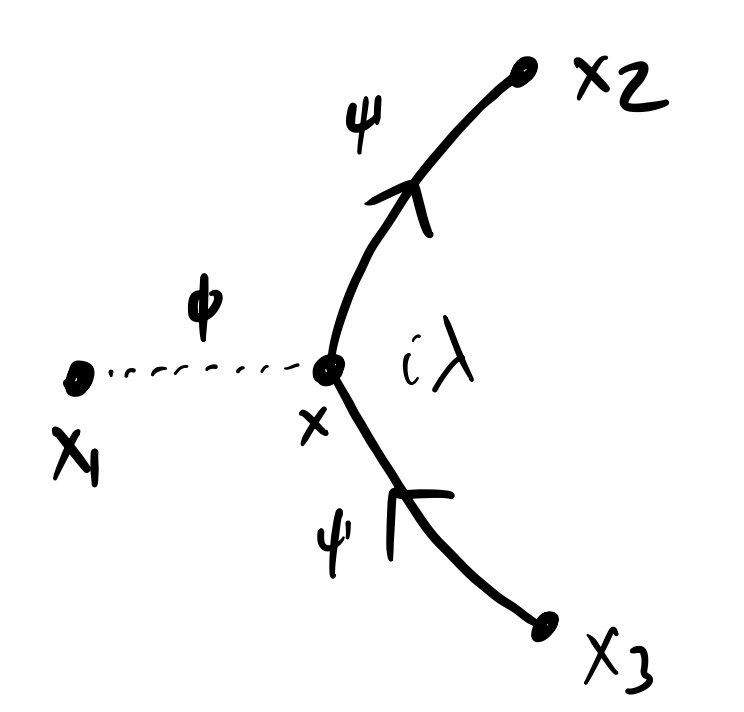
\includegraphics[scale=0.35]{Lectures/Images/lec6-xfeynman.png}
\end{center}

Or in momentum space:
\begin{equation}
    \avg{\phi_p\psi \bar{\psi}_{p'}} = i\lambda G_\phi(p)G_{\psi}(p + p')G_\psi(p') = i\lambda \frac{-i}{p^2 +M^2}\frac{-i}{\slashed{p} + \slashed{p}' + m}\frac{-i}{\slashed{p}' + m}
\end{equation}

\begin{center}
    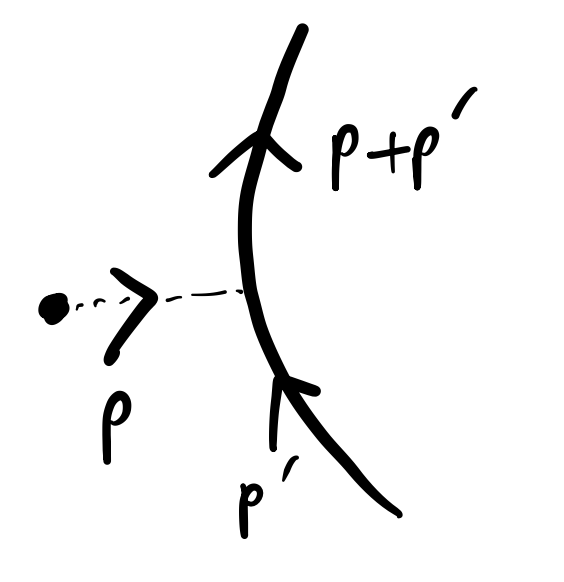
\includegraphics[scale=0.35]{Lectures/Images/lec6-pfeynman.png}
\end{center}


The amputated correlator $\avg{\phi_p\psi\bar{\psi}_{p'}}_{\text{amp}} = i\lambda\II$ will be related through LSZ to the 1$\to$2 S-matrix, namely the decay of a scalar particle into an electron/positron pair. When is the scalar particle unstable? If we imagine this in the rest frame of the scalar particle, this process requires $M > 2m$ (to produce the fermion and its antiparticle pair, plus giving the two kinetic energy) - when this condition is met $\phi$ is unstable, allowing for $\phi \to e^-e^+$, with decay rate $\Gamma \sim \lambda^2$ (which you will compute in PS4). 

\begin{center}
    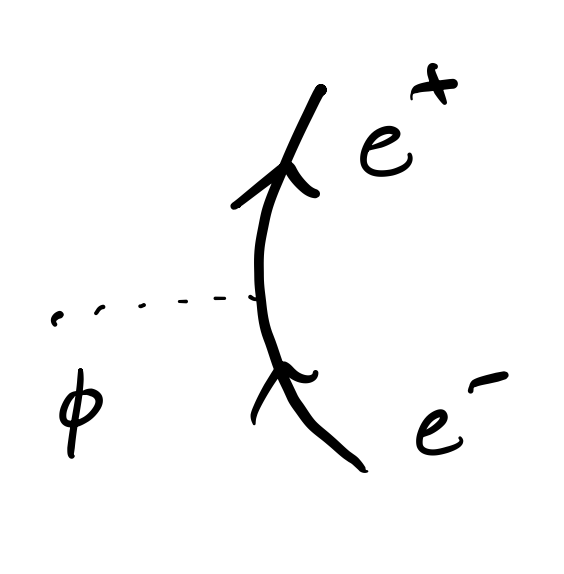
\includegraphics[scale=0.35]{Lectures/Images/lec6-scattering.png}
\end{center}

The decay rate also enters into the self-energy of the scalar, from which it is evident that $\Gamma \sim \lambda^2$.

\begin{center}
    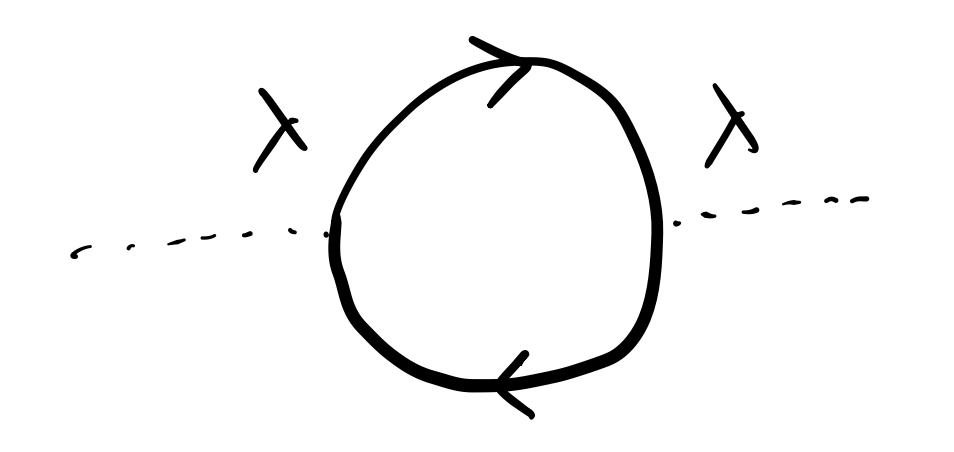
\includegraphics[scale=0.35]{Lectures/Images/lec6-selfenergy.png}
\end{center}

\subsection{Heavy Scalar Limit of Yukawa Theory - Fermi EFT}
Taking the limit where $M$ is huge (larger beyond all other energy scales), we can study its effects by integrating it out. Our full QFT has the generating functional:
\begin{equation}
    Z = \int \mathcal{D}\psi^\dag \mathcal{D}\psi \mathcal{D}\phi e^{i\int \bar{\psi}(i\slashed{p} - m)\psi + \lambda \phi \bar{\psi}\psi - \frac{1}{2}\phi(\p^2 + M^2)\phi}
\end{equation}
Note that if we just look at the $\phi$s (i.e. the $\phi$-sector), this is actually just a Gaussian theory! In our ultra-heavy limit, the mass energy is much greater than the kinetic term, so we neglect $\frac{1}{2}\phi(\p^2)\phi$. Thus, writing the $\phi$-part as:
\begin{equation}
    -\frac{1}{2}(\phi - \frac{\lambda}{M^2}\bar{\psi}\psi)M^2\left(\phi - \frac{\lambda}{M^2}\bar{\psi}\psi\right) + \frac{1}{2}\frac{\lambda}{M^2}\bar{\psi}\psi \bar{\psi}\psi
\end{equation}
Thus writing $\tilde{\phi} = (\phi - \frac{\lambda^2}{M^2}\bar{\psi}\psi)$, the above becomes:
\begin{equation}
    Z = \left(\int \mathcal{D}\tilde{\phi} e^{-\frac{1}{2}\tilde{\phi}M\tilde{\phi}}\right)\int \mathcal{D}\psi^\dag \mathcal{D}\psi e^{i\int \bar{\psi}(i\slashed{p} - m)\psi + \frac{1}{2}\frac{\lambda^2}{M^2}\bar{\psi}\psi\bar{\psi}\psi}
\end{equation}
So we can see that the $\phi$ generated an effective 4-fermion interaction! Free fermions do not scatter, but we have the emergence of an interaction vertex, mediated by the $\phi$ particle (which creates an effective interaction $ig_{\text{eff}} = i\frac{\lambda^2}{M^2}$); we can picture this as:

\begin{center}
    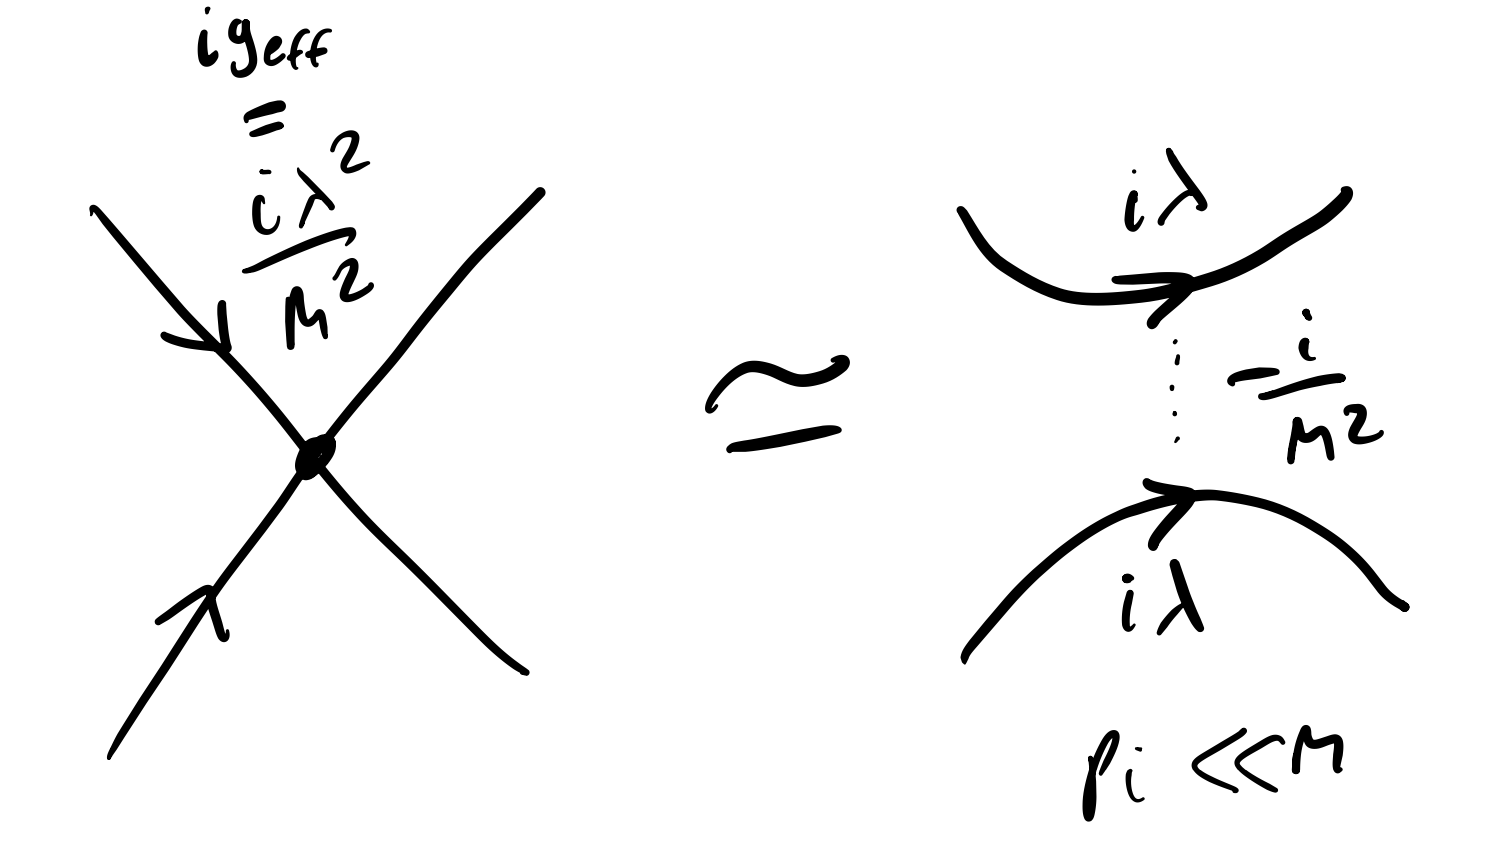
\includegraphics[scale=0.3]{Lectures/Images/lec6-effectiveinteraction.png}
\end{center}

This was the first effective theory considered - this is Fermi's effective field theory (EFT) of weak interactions, to explain $\beta$-decay. Radioactive materials emit electrons from time to time, with more specifically a neutron decaying into an electron, proton, and neutrino. This requires a 4-fermion interaction $g\bar{\psi}_1\psi_2\bar{\psi}_3\psi_4$. The microscopics of the theory came later, but the first try at explaining this phenomena was this EFT.

\begin{center}
    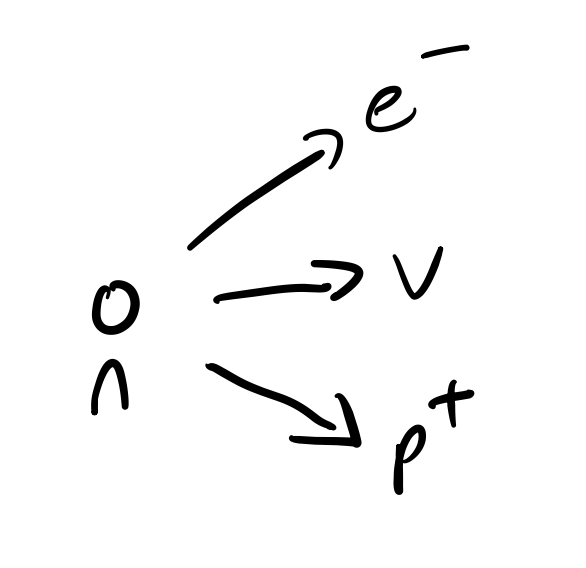
\includegraphics[scale=0.3]{Lectures/Images/lec6-neutrondecay.png}
\end{center}

This $\psi\bar{\psi}\psi\bar{\psi}$ interaction is irrelevant, or non-renormalizable. This is an energy that shrinks at small energies/IR and grows at high energies/UV. It is thus not UV complete, and cannot be the microscopic description of the theory. For us, the ``UV completion'' is the Yukawa theory (in Fermi's case it was a little more complicated, e.g. with Gauge fields). This effective interaction can be thought of as a force between particles (here the fermions $e^-, e^+$) that is mediated by the mysterious heavy particle. We can literally write this interaction as a potential:
\begin{equation}
    \begin{split}
        H_{\text{int}} &= -\frac{\lambda^2}{2M^2}\int d^4x \bar{\psi(x)}\psi(x)\bar{\psi}(x)\psi(x)
        \\ &=\int d^4xd^4y \bar{\psi(x)}\psi(x)V(x-y)\bar{\psi}(y)\psi(y)
    \end{split}
\end{equation}
where:
\begin{equation}
    V(x-y) = -\frac{\lambda^2}{2M^2}\delta^4(x-y)
\end{equation}
is a local interaction. In the problem set, you will find that this interaction is not a delta function (it is just sharply peaked), but in this extreme limit we currently consider, it is completely local. Given a particle at $x'$, because $V < 0$, it is energetically favourable to place another particle nearby. The Yukawa potential allows scalar particles to generate attractive interactions between fermions.

A final comment; if we spell out $\bar{\psi}\psi$, we find:
\begin{equation}
    \bar{\psi}\psi \sim b^\dag b + d^\dag d.
\end{equation}
Thus, all the particles - both fermions and anti-fermions attract each other. Phrased another way:
\begin{equation}
    H_{\text{int}} \sim \int_{xx'}(n_b + n_d)_xV(x - x')(n_b + n_d)_{x'}
\end{equation}
This is \emph{not} how we see electrons behave (which of course repulse), which indicates to us that the scalar particle is not what mediates the force between electrons. Instead, in QED we have that the force between electrons is mediated by the photon/gauge field\footnote{This wins out over the scalar mediation, as the photon is massles (and hence can mediate a long-range interaction), compared to the scalar mediated interaction which is short-ranged} $A_\mu$. This does not couple $\bar{\psi}, \psi$, but rather couples the current $j^\mu = \bar{\psi}\gamma^\mu \psi$, and in particular:
\begin{equation}
    \bar{\psi}\gamma^0 \psi = b^\dag b - d^\dag d
\end{equation}
So in QED:
\begin{equation}
    H_{\text{int}} \sim -\int_{xx'}(n_b - n_d)_xV(x - x')(n_b - n_d)_{x'}
\end{equation}
which means particles of the same charge repel, and particles of opposite charge attract. We will return to this soon!

Q (from me): Is it possible to look at the opposite limit where $2m \gg M$ (i.e. where the fermions are much heavier than the scalar), and integrate out the fermions, since the fermion subsector of the Yukawa Lagrangian is also Gaussian?

A (Luca): Yes; but note that this generates diagrams to all powers/orders of $\phi$, so is quite complicated. But, this is what people do, e.g., when they do quantum monte carlo simulations, because fermions are in general difficult to simulate (presumably due to sign problems).